\documentclass[border=10pt]{standalone}
\usepackage{pgfplots}
\pgfplotsset{compat=1.18}
\begin{document}
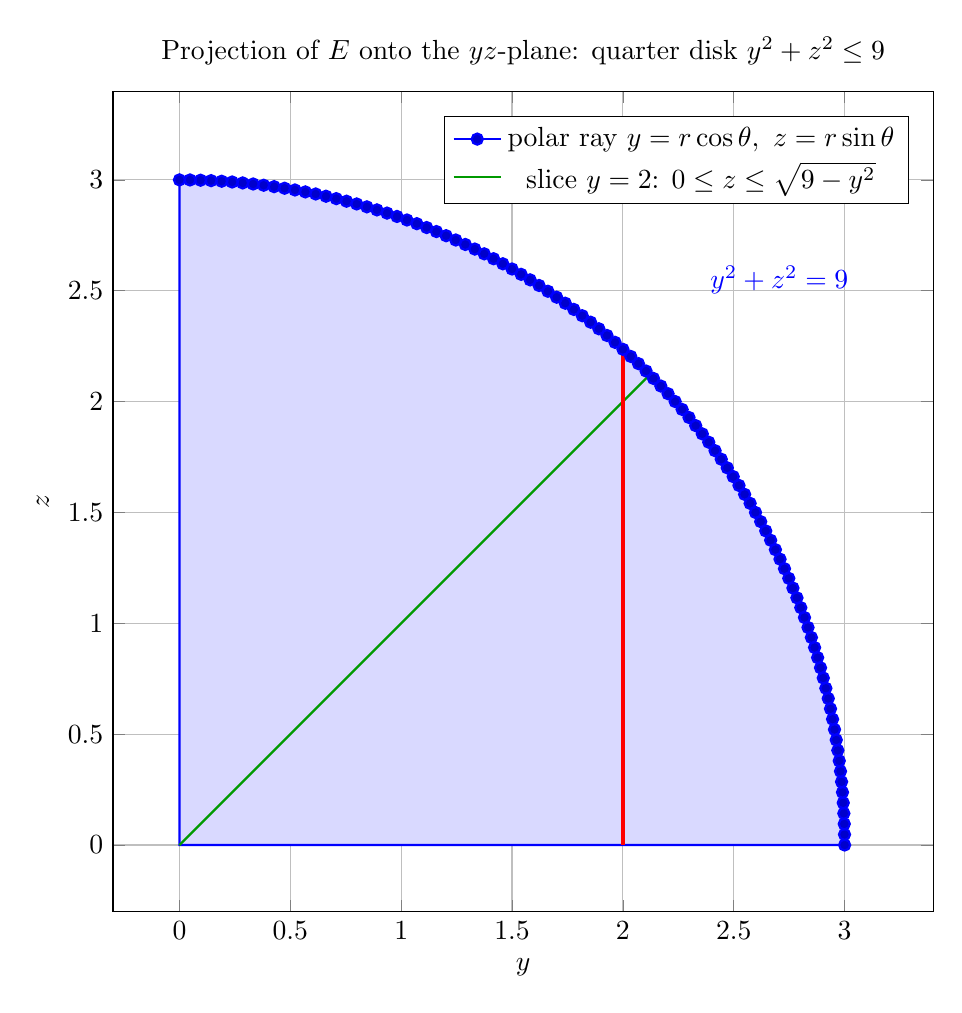
\begin{tikzpicture}
\begin{axis}[
    width=12cm, height=12cm,
    xlabel={$y$}, ylabel={$z$},
    xmin=-0.3, xmax=3.4, ymin=-0.3, ymax=3.4,
    axis equal image,
    grid,
    title={Projection of $E$ onto the $yz$-plane: quarter disk $y^2+z^2\le 9$},
    legend pos=north east,
]
% Quarter disk fill
\addplot+[domain=0:90, samples=100, draw=blue, fill=blue!15, thick]
({3*cos(x)}, {3*sin(x)}) \closedcycle;
% Polar ray
\addplot[green!60!black, thick] coordinates {(0,0) (2.1213,2.1213)};
\addlegendentry{polar ray $y=r\cos\theta,\ z=r\sin\theta$}
% Slice at y = 2
\addplot[red, very thick] coordinates {(2,0) (2,2.2361)};
\addlegendentry{slice $y=2$: $0\le z\le\sqrt{9-y^2}$}
% Arc label
\node[anchor=west, blue] at (axis cs:2.35,2.55) {$y^2+z^2=9$};
\end{axis}
\end{tikzpicture}
\end{document}
